\documentclass[a4paper,12pt]{article}

\usepackage[T1]{fontenc}
\usepackage[utf8]{inputenc}
\usepackage[english, polish]{babel}
\usepackage{lmodern}
\usepackage{graphicx}
\usepackage{fancyhdr}
\usepackage{float}
\usepackage{array}

%\usepackage{mathtools}


\setlength{\textheight}{23.5cm}
\setlength{\textwidth}{15.92cm}
\setlength{\footskip}{10mm}
\setlength{\oddsidemargin}{0mm}
\setlength{\evensidemargin}{0mm}
\setlength{\topmargin}{0mm}
\setlength{\headsep}{15mm}
\setlength{\parindent}{0cm}
\setlength{\parskip}{2.5mm}
%nowa extra row do tabeli :)  :) 
\setlength{\extrarowheight}{4pt}

\author{Justyna Ilczuk, Jacek Rosiński}

\begin{document}

\begin{center}

    \begin{tabular}{ | m{5cm}| m{5cm} | m{5cm} |}
    \hline 
    \multicolumn{2}{|c|}{{ \Large \textbf{Laboratorium Fizyki 2}} }
    &  
    \begin{center}
    Data wykonania ćwiczenia:
    \end{center}
    \begin{center}
      9.10.2013 
    \end{center}
    \begin{center}
    Środa 9.45-12.45
    \end{center}
     \\ 
    
    \hline
    \multicolumn{2}{|c|}{Justyna Ilczuk \newline Jacek Rosiński}
    & \begin{center}
    {\small Data złożenia sprawozdania:} \newline \today
    \end{center}   \\
   	
   	\hline
    Wydział Fizyki & Grupa: K-1 \newline Rok akademicki: 2013/2014 &    Nr ćwiczenia: 7 \\
   	\hline
   	\multicolumn{2}{|l|}{Prowadzący: Piotr Panecki} & \multicolumn{1}{|l|}{Ocena końcowa:}\\
    \hline
    \end{tabular}
\end{center}

\newpage

\pagestyle{fancy}
\fancyfoot[CO]{\ }
\fancyhead[RO]{\footnotesize{\thepage} }
%\fancyhead[RO]{\footnotesize{\ } }
\fancyhead[LO]{Justyna Ilczuk i Jacek Rosiński K-1, Dyfrakcja fali świetlnej na fali ultradźwiękowej }


\section{Cel ćwiczenia}

Celem ćwiczenia było zbadanie zjawisk jakie towarzyszą przejściu fali świetlnej przez ośrodek o zmiennym współczynniku załamania wywołanym falami ultradźwiękowymi. 

\section{Wstęp}

% wrzucanie wykresów:

%\begin{figure} [H]
%  \begin{center}
%    \includegraphics[width = 10cm]{../Obrazki_i_tekst/obrobione/u3.png}
%    \caption{Układ 3}
%  \end{center}
%\end{figure}

Eksperyent polegał na zbadaniu zjawisk jakim ulega fala świetlna przechodząc przez materiał o zmiennym współczynniku załamania. Zmienny współczynnik załamania został wywołany poprzez wykorzytanie zjawiska elektrostrykcji do wytworzenia stojącej fali ultradźwiękowej w wodzie, co można opisać następująco: 

$$ n(y,t) = n_0+\Delta n \cdot \cos (\Omega\cdot  t-K\cdot y) $$ 
$$ \Delta n = \Theta \cdot \sqrt{\frac{P_a}{\Pi \cdot R^2}}   $$
gdzie: \newline
$K$ - wektor falowy równoległy do osi $y$, 

$\Omega$ - częstotliwość kołowa,  

$\Theta$ - pewna stała zależna od parametrów materiałowych,
 
$P_a$ - moc fali ultradźwiękowej w cieczy,

$R$ - promień przewodnika,

$n_0$ - współczynnik załamania cieczy bez zaburzeń.



W eksperymencie mogliśmy mieć do czynienia z dwoma rodzajami dyfrakcji:
\begin{itemize}
\item dyfrakcją Ramana-Natha
\item dyfrakcją Bragga
\end{itemize}

Rodzaj dyfrakcji można określić na podstawie parametru Kleina-Cooke'a, który wyraża się następującym wzorem

\(
Q = \frac{K^2  L}{k cos \alpha }
\)
\\
Gdzie
\(
K = \frac{2 \pi}{ \Lambda }; \\ k = \frac{2 \pi}{\lambda}
\) wektory falowe fal: ultradźwiękowej i świetlnej

\( L  \) - długość wnęki

Jeżeli \( Q << 1\) to mamy do czynienia z dyfrakcją Ramana-Nata

Jeżeli \( Q >> 1 \) to mamy do czynienia z dyfrakcją Bragga

% Nie piszmy we wstępie co nam wyszlo jako całość...
%%
%W eksperymenicie wszystkie wartości $Q$ były dużo mniejsze od 1, więc mieliśmy do czynienia z dyfrakcją Ramana-Natha, która polega na tym, że fala przechodząc przez ośrodek o periodyczznych zmianach współczynnika załamania zaburza swój front falowy, który następnie ulega dyfrakcji podobne jak na siatce dyfrakcyjnej. Stosujemy więc wzór: 
%
Wzór dyfrakcyjny dla dyfrakcji Ramana-Natha:

$$ \frac{m \cdot \lambda}{\Lambda}=\sin (\alpha) $$
gdzie: \\
$\lambda$ - długość fali lasera, 
$m$ - numer prążka liczony od środkowego prążka z numerem 0, 
$ \alpha $ - kąt zakreślany między prażkiem z numerem 0 i prążkiem m-tym,
% NO TO MOŻE BYĆ ŹLE....  
$ \Lambda $ - stała siatki dyfrakcyjnej. W tym przypadku połówka długości fali ultradźwiękowej. \\

Długość fali ultradźwiękowej mogliśmy wyznaczyć na kilka sposobów:
\begin{enumerate}
  \item Poprzez odczytanie częstotliwości z częstotliwościomierza  i obliczenie z wzoru: $\Lambda=\frac{v}{f}$, korzystając z tablicowej watrości prędkości dźwięku w wodzie, jaką znalieźliśmy na stronie podanej w żrółach na końcu sprawozdania. 
  \item Poprzez manewry długością wnęki rezonansowej i ręczne odczytywanie kolejnych maksimów jako kolejnych połówek długości fali ultradźwiękowej.
  \item Poprzez zastosowanie wzoru dla siatki dyfrakcyjnej $\Lambda=\frac{m \cdot \lambda}{\sin (\alpha)}$
\end{enumerate}

Podstawowa zależność dla prędkości fali wynosi: 

$$v = \frac{\omega}{k} = \frac{2\cdot \pi \cdot f }{\frac{2\cdot \pi}{\Lambda} }= \Lambda \cdot f $$

Zgodnie na tak niskim zakresie fal ultradźwiękowych spodziewaliśmy się krzywej dyspersji przypominającą linię prostą. Dla tego też wyznaczone długości fali z danych tablicowych uważamy za wzorcowe. 



Aby sprawdzić powyższą hiptezę używaliśmy testu $\chi^2$ zgodnie z poniższym wzorem. 
$$
\chi^2 = \Sigma_{i=1}^n {\left( \frac{y_i - f(x_i)}{\sigma_i} \right)}^2
$$
Gdzie $y_i$ to nasze wybiki, zaś $f(x_i)$ to wyniki pochodzące z dopasowanej prostej. $\sigma_i$ to niepewności pomiarów. 
$\chi^2$ po zsumoawniu odpowiada na pytanie czy hipoteza, jaką stawiamy jest prawdziwa: 
\begin{itemize}
  \item $\chi^2 \gg 1$ - hipoteza przez nas postawiona jest fałszywa 
  \item $\chi^2 \approx 1$ - hipoteza jest zgodna z doświadczeniem
\end{itemize}


\section{Użyty sprzęt i układy pomiarowe}


% tutaj trzeba wrzucić schemat układu pomiarowego i opis użytych przyrządów
% a także szczegóły techniczne, specyficzne dla naszego setupu eksperymentu

Do przeprowadzenia eksperymenty używaliśmy: 

\begin{enumerate}
  \item Lasera czerwonego ( 632.8 nm , 1mW ) 
  \item Zwierciadeł i soczewek do doprowadzenia wiązki i wydłużenia drogi optycznej światła
  \item Generatora G-35
  \item Częstotliwościomierza PFL-30
  \item Suwmiarki, metrówki i linijki  
  \item Śruby mikrometrycznej wraz z rezonatorem fali ultradźwiękowej
\end{enumerate}

Żeby wziększyć dokładność pomiarów, poszerzyliśmy wiązkę lasera używając do tego prostego układu optycznego.\\
Ze względu na ograniczoną powierzchnię laboratorium fizyki 2, do wydłurzenia drogi lasera po przejściu przez rezonator użyliśmy zwierciadeł wydłurzając drogę wiązki do $732cm$. 

Schemat układu pomiarowego przedstawiony jest poniżej: 

\begin{figure} [H]
  \begin{center}
    \includegraphics[width = 15cm]{Rysunek.png}
    \caption{Układ pomiarowy}
  \end{center}
\end{figure}



\section{Opracowanie wyników}

Niepewności jakie przyjęliśmy to:
\begin{enumerate}
  \item Niepewność pomiaru drogi optycznej: 3cm 
  \item Niepewność pomiaru śrubą mikrometryczną: 0.2 mm 
  \item Niepewność pomiaru suwmiarką: 0.1 cm 
  
\end{enumerate}

Uzasadniamy je tym, że przy każdym mierzonym parametrze do niepewności urządzenia dochodził błąd związany z dokładnością wyznaczenia parametru, jak na przykład wyśrodkowania suwmiarki na konkretne mierzone punkty. Wyśrodkowania śruby na odpowiednie maxima (powstanie fali stojącej w wodzie). Złożoność drogi optycznej dla promieni lasera. 

Aby zmiejszyć niedokładność pomiarów zliczaliśmy wzmocnienia fali świetlnej dla maksymalnej ilości prążków, dzięki czemu pomiar suwniarką był dokładniejszy. Niestety pomiar śrubą mikrometryczną okazał się bardzo wadliwy. Przy pomiarze tym prawdopodobnie kolkakrotnie popełnialiśmy błędy związanie z wyznaczeniem maskimum. Wyniki przedstawiamy w poniższej tabelce: 


\begin{figure} [H]
  \begin{center}
    \includegraphics[width = 10cm]{tab1.png}
    \caption{Pomiary odległości między maksimami maksymalnego obserwowanego rzędu od częstotliwości}
  \end{center}
\end{figure}

Natomiast wyniki pomiarów śrubą mikrometryczną zamieszczamy w poniższej tabeli: 

\begin{figure} [H]
  \begin{center}
    \includegraphics[width = 10cm]{tab2.png}
    \caption{Odległościami wyznaczone pomiarem na śrubie mikrometryczenj. Wszyskie wielkości podano w [mm]}
  \end{center}
\end{figure}


Następnie przyjmując tablicową wartość prędkości dźwieku w wodzie i na podstawie odczytu częstotliwości wyznaczyliśmy długości fali ultradźwiękowej. Wyniki przedstawia tabela: 

\begin{figure} [H]
  \begin{center}
    \includegraphics[width = 5cm]{tab3.png}
    \caption{Tablicowe długości fali dźwiękowej w wodzie}
  \end{center}
\end{figure}

Wyznaczone powyżej wielkości służyły nam jedynie orientacyjnie do porównywania wyników. 

Kolejnym sposobem wyliczenia było podstawienie do wzoru na dyfrakcję na siatce. Wyniki przedstawiamy w tabelce: 

\begin{figure} [H]
  \begin{center}
    \includegraphics[width = 5cm]{tab4.png}
    \caption{Długość fali liczona za pomocą wzoru na dydrakcję na siatce}
  \end{center}
\end{figure}

Ową zależność przedstawia również wykres: 

\begin{figure} [H]
  \begin{center}
    \includegraphics[width = 12cm]{wykres1.png}
    \caption{Zależność długości fali od częstotliwości}
  \end{center}
\end{figure}

Niepewność z pomiarów śrubą mikrometryczną wyliczono dodając kwadraty poszczególnych błędów pod pierwiastkiem natomiast długości fali liczonej z wzoru na dyfrakcję na siatce, z różniczki zupełnej. Niepewności długości fali wyznaczanej z danych tablicowych zestawiono dla porównania jak również średnią selektywną. Owe wyniki przedstawia tabela: 


\begin{figure} [H]
  \begin{center}
    \includegraphics[width = 17cm]{tab5.png}
    \caption{Porównanie długości fal wyznacznych różnymi metodami}
  \end{center}
\end{figure}

Na podstawie powyższych danych mogliśmy rozpatrywać rodzaj dyfrakcji z jaką mieliśmy do czynienia i jak wspominalismy wcześniej okazało się że była to dyfrakcja Ramana-Natha. Wyliczone parametry  przedstawia poniższa tabela: 

\begin{figure} [H]
  \begin{center}
    \includegraphics[width = 3cm]{tab6.png}
    \caption{Parametry Kleina-Cooke'a}
  \end{center}
\end{figure}

Dalej wyliczyliśmy zależność prędkości fali ultradźwiękowej od częstotliwości. Wyniki zamieszczamy poniżej: 

\begin{figure} [H]
  \begin{center}
    \includegraphics[width = 10cm]{tab7.png}
    \caption{Prędkości fali ultradźwiekowej}
  \end{center}
\end{figure}


\begin{figure} [H]
  \begin{center}
    \includegraphics[width = 7cm]{wykres5.png}
    \caption{Prędkość dźwięku w wodzie}
  \end{center}
\end{figure}


Jako null hipotezę przyjęliśmy, że prędkość dzwięku w wodzie jest stała. Dopasowana krzywa jest prostą o współczynniku $a=1523(40)$. Co daje nam prędkość równą $1523(40) \frac{m}{s}$
Wynik $\chi^2$ wyniósł: 8.3, co daje nam wartość poziomu istotności 0.3, co nie pozwala nam odrzucic zerowej hipotezy.

\section{Wnioski}


Parametr Kleina-Cooke'a określił, że w doświadczeniu mieliśmy do czynienia z dyfrakcją Ramana-Natha. 

Wyliczyliśmy, że prędkość fali dźwiękowej w wodzie jest stała niezależnie od częstotliwości i wynosi $1523(40) \frac{m}{s}$ i zgadza się z danymi tablicowymi.


\section {Źródła dodatkowe}
  
 \begin{itemize}
   \item prędkość dźwięku w wodzie: $ 1482 m/s$ \\ http://fatcat.ftj.agh.edu.pl/~kaprzyk/Fizyka/fizyka/node102.html
   \item A SIMPLE AND ACCURATE FORMULA FOR THE SOUND VELOCITY IN WATER	J. Lubbers, R. Graaff, University of Groningen
   
 \end{itemize}

\end{document}
